\subsection*{Taxas relacionadas}
\subsection*{Máximos e Mínimos}
\begin{tcolorbox}
\begin{defi}
Seja $f:X\longrightarrow \mathbb{R}$ e $c\in X$ então $f(c)$ é o
\begin{itemize}
    \item valor \textbf{máximo absoluto} de $f$ em $X$ se $f(c)\geq f(x)$ para todo $x$ em $X$.
    \item valor \textbf{mínimo absoluto} de $f$ em $X$ se $f(c)\leq f(x)$ para todo $x$ em $X$.
\end{itemize}
\end{defi}
\begin{defi}
Seja $f:X\longrightarrow \mathbb{R}$ e $c\in X$ então o número $f(c)$ é um
\begin{itemize}
    \item valor \textbf{máximo local} de $f$ se $f(c)\geq f(x)$ para valores de $x$ próximos de $c$.
    \item valor \textbf{mínimo local} de $f$ se $f(c)\leq f(x)$ para valores de $x$ próximos de $c$.
\end{itemize}
\end{defi}
\begin{teorema}
Seja $f:[a,b]\longrightarrow\mathbb{R}$ contínua. Então $f$ assume máximo e mínimo absoluto em $[a,b]$.
\end{teorema}
\begin{teorema}
Se $f$ tiver um \textbf{máximo} ou \textbf{mínimo} local em $c$ e se $f'(c)$ existir, então $f'(c)=0$.
\end{teorema}
\begin{defi}
Seja $f:X\longrightarrow \mathbb{R}$. Dizemos que um número $c \in X$ é um \textbf{número crítico} de $f$ se $f'(c)=0$ ou $f'(c)$ não existe.
\end{defi}
\begin{prop}
Se $f$ tiver um \textbf{máximo} ou \textbf{mínimo} local em $c$, então $c$ é um número crítico de $f$.
\end{prop}
\end{tcolorbox}

\subsection*{Teoremas de Rolle e do Valor Médio}
\begin{tcolorbox}
\begin{teorema}[Teoremas de Rolle] Aqui vem o texto do Teorema

\begin{figure}[H]
    \centering
    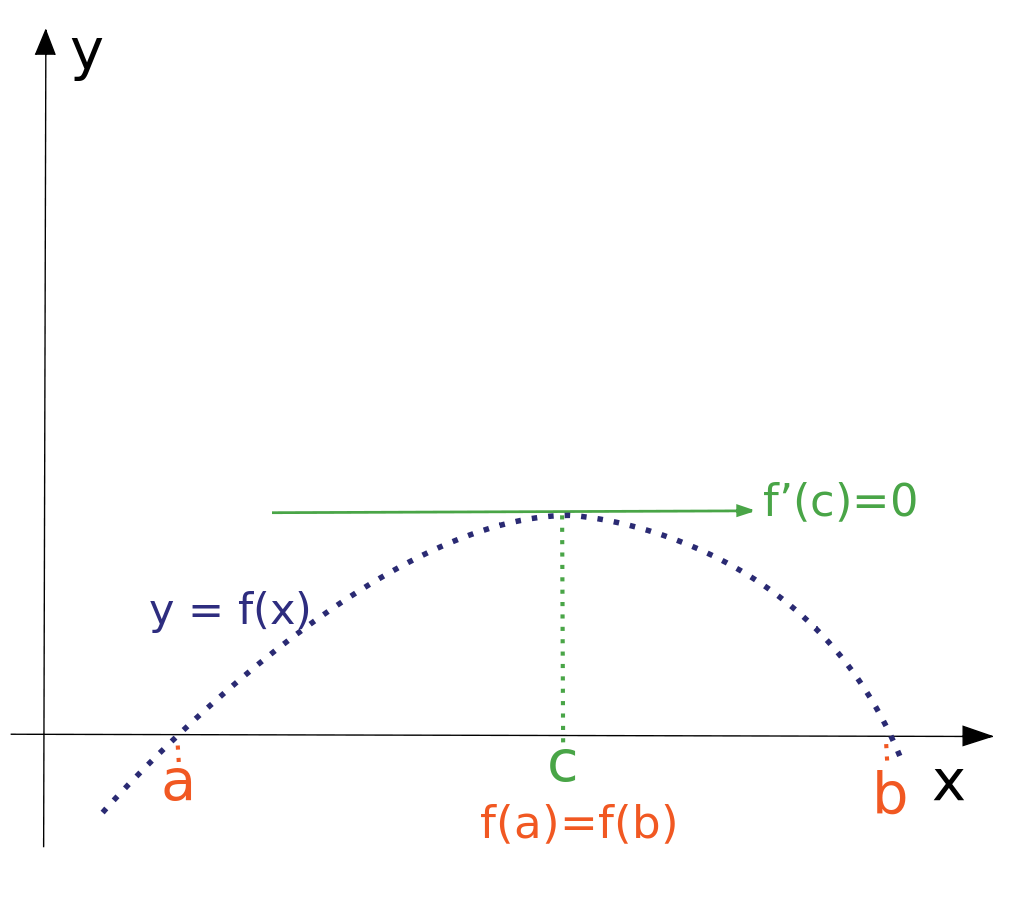
\includegraphics[scale=0.25, height=100px]{Figuras/rolle.png}
\end{figure}
\end{teorema}
\begin{teorema}[Valor Médio]

\end{teorema}
\end{tcolorbox}
\subsection*{Região de crescimento e concavidade. Esboço de gráficos}

\subsection*{ O Teorema de Taylor; a aproximação polinomial. }
\subsection*{Problemas de otimização}
\subsection*{Regra de L'Hospital}
\begin{tcolorbox}
Se $\lim\limits_{x\to a}\dfrac{f(x)}{g(x)}=\dfrac{0}{0} \text{ ou } \dfrac{\pm\infty}{\pm\infty}$ então
\begin{align*}
    \lim\limits_{x\to a}\dfrac{f(x)}{g(x)}=\lim\limits_{x\to a}\dfrac{f'(x)}{g'(x)}.
\end{align*}
\end{tcolorbox}